%           ******************************************************
%          **   course         : Memory Technologies             **
%         ***   Presentation   : 01                              ***
%        ****   Topic          : UMA and NUMA Architecture       ****
%        ****   AUTHOR         : Reza Adinepour                  ****
%         ***   Student ID:    : 402131055                       ***
%          **   Github         : github.com/rezaAdinepour/       **
%           ******************************************************

\documentclass[
	12pt, % Set the default font size, options include: 8pt, 9pt, 10pt, 11pt, 12pt, 14pt, 17pt, 20pt
	%t, % Uncomment to vertically align all slide content to the top of the slide, rather than the default centered
	%aspectratio=169, % Uncomment to set the aspect ratio to a 16:9 ratio which matches the aspect ratio of 1080p and 4K screens and projectors
]{beamer}

\graphicspath{{Images/}{./}} % Specifies where to look for included images (trailing slash required)

\usepackage{booktabs} % Allows the use of \toprule, \midrule and \bottomrule for better rules in tables
\usepackage{subcaption}


%----------------------------------------------------------------------------------------
%	SELECT LAYOUT THEME
%----------------------------------------------------------------------------------------

% Beamer comes with a number of default layout themes which change the colors and layouts of slides. Below is a list of all themes available, uncomment each in turn to see what they look like.

\usecolortheme{beaver}
\usetheme{Madrid}
\setbeamercolor{section in head/foot}{bg=black}
\setbeamercolor{title}{fg=white, bg=black}
\setbeamercolor{frametitle}{fg=white,bg=black}
\setbeamercolor{block title}{fg=white,bg=black}
\setbeamercolor{item}{fg=black}
\setbeamertemplate{navigation symbols}{}
\setbeamercovered{transparent}

% Add these lines to set the bottom bar to black
\setbeamercolor{author in head/foot}{bg=black, fg=white}
\setbeamercolor{title in head/foot}{bg=gray, fg=white}
\setbeamercolor{date in head/foot}{bg=black, fg=white}
\setbeamercolor{headline}{bg=black}
\setbeamercolor{footline}{bg=black}


%----------------------------------------------------------------------------------------
%	SELECT FONT THEME & FONTS
%----------------------------------------------------------------------------------------

% Beamer comes with several font themes to easily change the fonts used in various parts of the presentation. Review the comments beside each one to decide if you would like to use it. Note that additional options can be specified for several of these font themes, consult the beamer documentation for more information.

\usefonttheme{default} % Typeset using the default sans serif font
%\usefonttheme{serif} % Typeset using the default serif font (make sure a sans font isn't being set as the default font if you use this option!)
%\usefonttheme{structurebold} % Typeset important structure text (titles, headlines, footlines, sidebar, etc) in bold
%\usefonttheme{structureitalicserif} % Typeset important structure text (titles, headlines, footlines, sidebar, etc) in italic serif
%\usefonttheme{structuresmallcapsserif} % Typeset important structure text (titles, headlines, footlines, sidebar, etc) in small caps serif

%------------------------------------------------

%\usepackage{mathptmx} % Use the Times font for serif text
\usepackage{palatino} % Use the Palatino font for serif text

%\usepackage{helvet} % Use the Helvetica font for sans serif text
\usepackage[default]{opensans} % Use the Open Sans font for sans serif text
%\usepackage[default]{FiraSans} % Use the Fira Sans font for sans serif text
%\usepackage[default]{lato} % Use the Lato font for sans serif text

%----------------------------------------------------------------------------------------
%	SELECT INNER THEME
%----------------------------------------------------------------------------------------

% Inner themes change the styling of internal slide elements, for example: bullet points, blocks, bibliography entries, title pages, theorems, etc. Uncomment each theme in turn to see what changes it makes to your presentation.

%\useinnertheme{default}
\useinnertheme{circles}
%\useinnertheme{rectangles}
%\useinnertheme{rounded}
%\useinnertheme{inmargin}

%----------------------------------------------------------------------------------------
%	SELECT OUTER THEME
%----------------------------------------------------------------------------------------

% Outer themes change the overall layout of slides, such as: header and footer lines, sidebars and slide titles. Uncomment each theme in turn to see what changes it makes to your presentation.

%\useoutertheme{default}
%\useoutertheme{infolines}
%\useoutertheme{miniframes}
%\useoutertheme{smoothbars}
%\useoutertheme{sidebar}
%\useoutertheme{split}
%\useoutertheme{shadow}
%\useoutertheme{tree}
%\useoutertheme{smoothtree}

%\setbeamertemplate{footline} % Uncomment this line to remove the footer line in all slides
%\setbeamertemplate{footline}[page number] % Uncomment this line to replace the footer line in all slides with a simple slide count

%\setbeamertemplate{navigation symbols}{} % Uncomment this line to remove the navigation symbols from the bottom of all slides

%----------------------------------------------------------------------------------------
%	PRESENTATION INFORMATION
%----------------------------------------------------------------------------------------

\title[ReTransformer]{ReTransformer} % The short title in the optional parameter appears at the bottom of every slide, the full title in the main parameter is only on the title page

\subtitle{ReRAM-based Processing-in-Memory Architecture for Transformer Acceleration} % Presentation subtitle, remove this command if a subtitle isn't required

\author[Reza Adinepour]{Reza Adinepour} % Presenter name(s), the optional parameter can contain a shortened version to appear on the bottom of every slide, while the main parameter will appear on the title slide

\institute[AUT]{Amirkabir University of Technology (Tehran Polytechnic) \\ \smallskip \href{mailto:adinepour@aut.ac.ir}{\texttt{adinepour@aut.ac.ir}}} % Your institution, the optional parameter can be used for the institution shorthand and will appear on the bottom of every slide after author names, while the required parameter is used on the title slide and can include your email address or additional information on separate lines

\date[\today]{Computer Engineering Department \\ \today} % Presentation date or conference/meeting name, the optional parameter can contain a shortened version to appear on the bottom of every slide, while the required parameter value is output to the title slide

%----------------------------------------------------------------------------------------

\begin{document}

%----------------------------------------------------------------------------------------
%	TITLE SLIDE
%----------------------------------------------------------------------------------------

\begin{frame}
	\titlepage % Output the title slide, automatically created using the text entered in the PRESENTATION INFORMATION block above
	\centering
\includegraphics[scale=0.13]{Images/Logo/logo2.png}
\end{frame}

%----------------------------------------------------------------------------------------
%	TABLE OF CONTENTS SLIDE
%----------------------------------------------------------------------------------------

% The table of contents outputs the sections and subsections that appear in your presentation, specified with the standard \section and \subsection commands. You may either display all sections and subsections on one slide with \tableofcontents, or display each section at a time on subsequent slides with \tableofcontents[pausesections]. The latter is useful if you want to step through each section and mention what you will discuss.

\begin{frame}
	\frametitle{Presentation Overview} % Slide title, remove this command for no title
	
	\tableofcontents % Output the table of contents (all sections on one slide)
	%\tableofcontents[pausesections] % Output the table of contents (break sections up across separate slides)
\end{frame}

%----------------------------------------------------------------------------------------
%	PRESENTATION BODY SLIDES
%----------------------------------------------------------------------------------------

\section{Memory Architecture Overview}



\begin{frame}
	\frametitle{Memory Architecture Overview}
	\textbf{What is this structure?}\\
	--- Defines how computer memory is organized and accessed.\\
	\begin{enumerate}
		\item \textcolor{red}{U}niform \textcolor{red}{M}emory \textcolor{red}{A}ccess (UMA) 
		\item \textcolor{red}{N}on-\textcolor{red}{U}niform \textcolor{red}{M}emory \textcolor{red}{A	}ccess (NUMA)
		\item \textcolor{red}{C}ache-\textcolor{red}{O}nly \textcolor{red}{M}emory \textcolor{red}{A}ccess (COMA)
	\end{enumerate}
	
	\textbf{--- In this presentation we talk about UMA and NUMA Architecture}
\end{frame}




\subsection{Uniform Memory Access (UMA)}

\begin{frame}
	\frametitle{Uniform Memory Access (UMA)}
	
	\begin{figure}[h]
		\centering
		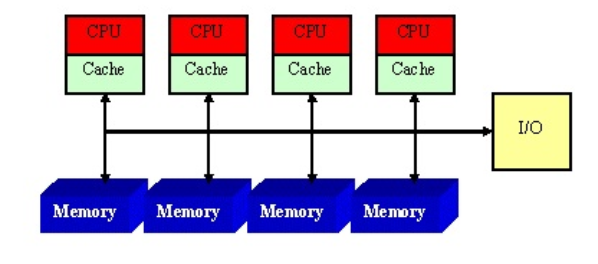
\includegraphics[width=0.8\linewidth]{Images/img1}
		\caption{Processors with equal access to memory}
		\label{Illustrates processors with equal access to memory.}
	\end{figure}
	
	\begin{enumerate}
		\item Same latency for all processors to access memory.
		\item Hardware cache typically present with each processor.
	\end{enumerate}	
\end{frame}





\begin{frame}
	\frametitle{Uniform Memory Access (UMA) (Cont.)}
	
	\begin{enumerate}
		\item Equal memory access for all processors.
		\item Shared memory, any processor can access any part at any time.
		\item Simple, cost-effective, highly scalable.
	\end{enumerate}
	
	\textcolor{green}{Advantages:}
	\begin{enumerate}
		\item \textbf{Ease of Implementation:} Minimal hardware modifications, cost-effective.
		\item \textbf{Scalability:} Easily scales with more processors without impacting access times.
	\end{enumerate}
	
	\textcolor{red}{Disadvantages:}
	\begin{enumerate}
		\item \textbf{Memory Contention:} Increased processors may lead to slower access times.
		\item \textbf{Limited Bandwidth:} Shared memory bus can become a bottleneck.
	\end{enumerate}


\end{frame}







\begin{frame}
	\frametitle{Uniform Memory Access (UMA) (Cont.)}
	
	Example System:
	\begin{enumerate}
		\item \textbf{Symmetric Multiprocessing (SMP) System: }
		\begin{enumerate}
			\item Multiple processors share common memory.
			\item Controlled by a single operating system.
			\item Common in servers and high-performance computing.
		\end{enumerate}
	\end{enumerate}
	
	Summary:
	\begin{enumerate}
		\item \textbf{\textcolor{green}{Strengths:} Simplicity and scalability.}
		\item \textbf{\textcolor{red}{Weaknesses:} Potential for memory contention and limited bandwidth in larger systems.}
	\end{enumerate}
	
\end{frame}










%------------------------------------------------


\subsection{Non-uniform Memory Access (NUMA)}

\begin{frame}
	\frametitle{Non-uniform Memory Access (NUMA)}
	
	
	
	\begin{figure}[h]
		\centering
		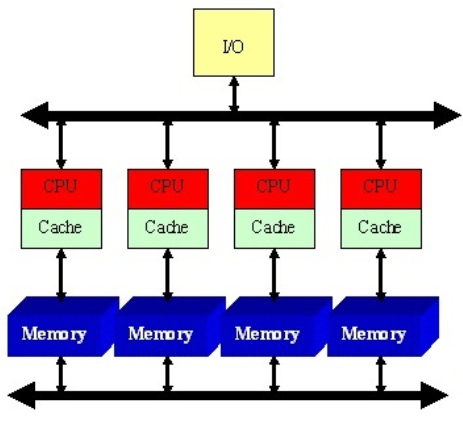
\includegraphics[width=0.5\linewidth]{Images/img2}
		\caption{Processors with equal access to memory}
		\label{Processors with local memory}
	\end{figure}
	
	\begin{enumerate}
		\item Each processor has its local memory.
	\end{enumerate}
	
	
\end{frame}


\begin{frame}
	\frametitle{Non-uniform Memory Access (NUMA) (Cont.)}
	
	\begin{enumerate}
		\item Memory divided into multiple banks, each processor has its local bank.
		\item Processors can access other banks, but at higher latency than local access.
		\item Efficient memory resource use, potential better performance than UMA for certain workloads.
	\end{enumerate}
	
	\textcolor{green}{Advantages:}
	\begin{enumerate}
		\item \textbf{Reduced Memory Contention:} Each processor has its local memory, minimizing contention.
		\item \textbf{Increased Memory Bandwidth:} Local memory banks lead to higher bandwidth than UMA.
		\item \textbf{Efficient Memory Use:} Allocation based on processor needs enhances resource utilization.
	\end{enumerate}
	
	
\end{frame}



\begin{frame}
	\frametitle{Non-uniform Memory Access (NUMA) (Cont.)}
	
	\textcolor{red}{Advantages:}
	\begin{enumerate}
		\item \textbf{Higher Implementation Complexity:} Additional hardware and software complexity.
		\item \textbf{Higher Latency for Remote Access:} Accessing remote memory incurs higher latency.
	\end{enumerate}
	
	Example System:
	\begin{enumerate}
		\item \textbf{Multi-Socket Server:}
		\begin{enumerate}
			\item Each socket has its processors and memory banks.
			\item Sockets connected via a high-speed interconnect.
			\item Commonly used in data centers, offers better performance for specific workloads.
		\end{enumerate}
	\end{enumerate}
\end{frame}



% -------------------------------------------------------------

\subsection{Cache-only Memory Access (COMA)}

% -------------------------------------------------------------











%------------------------------------------------
\section{Code Snippets}

\begin{frame}
	\frametitle{Code Snippets}
	
	\begin{quote}
		Run the \textcolor{blue}{code!}\\
		--- This code is generated by ChatGP
	\end{quote}
	
\end{frame}




%------------------------------------------------
\section{Differences between UMA and NUMA}

\begin{frame}
	\frametitle{Differences between UMA and NUMA}
	
	\begin{enumerate}
		\item \textbf{Memory access time: }
		\begin{enumerate}
			\item NUMA: \\ Memory access time varies depending on the location of the data in memory. Accessing data in the local memory of a processor is faster than accessing data in the memory of a remote processor.
			
			\item UMA: \\ Memory access time is uniform across all processors since they share the same memory pool.
		\end{enumerate}
		\item \textbf{Scalability: }
		\begin{enumerate}
			\item NUMA architecture is highly scalable and can support a large number of processors.
			
			\item UMA architecture is not as scalable as NUMA and may face performance issues when used with a large number of processors.
		\end{enumerate}
	\end{enumerate}
	
\end{frame}


%------------------------------------------------


%----------------------------------------------------------------------------------------
%	CLOSING SLIDE
%----------------------------------------------------------------------------------------

\begin{frame}[plain] % The optional argument 'plain' hides the headline and footline
	\begin{center}
		{\Huge The End}
		
		\bigskip\bigskip % Vertical whitespace
		
		{\LARGE Questions? Comments?}\\
		You can find this slides here:\\
		\textcolor{blue}{\href{https://github.com/M-Sc-AUT/M.Sc-Computer-Architecture/tree/main/Memory Technologies}{github.com/M-Sc-AUT/M.Sc-Computer-Architecture/Memory Technologies}}
	\end{center}
\end{frame}

%----------------------------------------------------------------------------------------

\end{document} 